\chapter{Appendix}
%Todo Add SAMPLE GAME XML
% Todo Add XSD
% Todo Add DTT ??
\textbf{Samplegame:}
\lstset{language=XML}
\begin{lstlisting}

<?xml version="1.0" encoding="UTF-8"?>
<adventure name="Dark trinity" entry="dungeon" story="You are alone. In front of you is a dark dungeon. Suddenly you hear some noise. RUN!">

    <!--Player -->
    <player name="Mike Moore" life="100" xcordinate="1" ycordinate="1">
        <item reference="knife" />
        <item reference="lamp" />
        <item reference="apple" />
    </player>

    <!--Items -->
    
    <equip-item
        id="knife"
        name="Knife"
        description="A sharp knife, use with caution!"
        damage="5" />

    <consum-item
        id="apple"
        name="Apple"
        description="A red apply. Seems to be tasty!"/>

    <collect-item
        id="lamp"
        name="Lamp"
        description="A bright lamp" />

    <!--Creatures -->

    <creature
        id="ghost"
        name="Dark ghost"
        description="A dangerous ghost"
        life="20"
        damage="10">
        <item ref="lamp"/>
    </creature>
       
    <!--Rooms -->

    <room id="dungeon" name="Dark Dungeon" width="3" height="3" message="You are alone. In front of you is a dark dungeon. Suddenly you hear some noise. RUN!">
        <door xcoordinate="2" ycoordinate="2" room="chamber" target="closeddoor" />
        <creature-ref reference="ghost" xcoordinate="2" ycoordinate="1" />
        <item-ref reference="apple" x="1" y="2" />
    </room>

    <room id="chamber" name="Chamber of horror" width="3" height="3" message="You are alone. Forever.">
        <door xcoordinate="0" ycoordinate="0" id="closeddoor"/>
        <creature-ref reference="ghost" xcoordinate="2" ycoordinate="1" />
    </room>

</adventure>
\end{lstlisting}
\textbf{XSD:}
\lstset{language=XML}
\begin{lstlisting}
<?xml version="1.0"?>

<xs:schema version="1.0"
           xmlns:xs="http://www.w3.org/2001/XMLSchema"
           elementFormDefault="qualified">

    <!-- Definiton of Types-->   
    <xs:simpleType name="idtype">
        <xs:restriction base="xs:string">
            <xs:pattern value="([a-z])*[0-9]"/>
        </xs:restriction>
    </xs:simpleType>
    
    <xs:simpleType name="gameString">
        <xs:restriction base="xs:string">
            <xs:pattern value="([a-zA-Z])*"/>
        </xs:restriction>
    </xs:simpleType>
    
    <!-- Definiton of simple Elements-->
    <xs:attribute name="name" type="gameString" use="required"/>
    <xs:attribute name="id" type="gameString" use="required"/>
    <xs:attribute name="reference" type="gameString" use="required"/>
    <xs:attribute name="description" type="xs:string"/>
    <xs:attribute name="message" type="xs:string"/>
    <xs:attribute name="life" type="xs:positiveInteger" use="required"/>
    <xs:attribute name="maxlife" type="xs:positiveInteger" use="required"/>
    <xs:attribute name="target" type="gameString" use="required"/>
    <xs:attribute name="destination" type="gameString" use="required" default="closeddoor"/>
    
    <xs:attributeGroup name="position">
        <xs:attribute name="xcordinate" type="xs:positiveInteger" use="required"/>
        <xs:attribute name="ycordinate" type="xs:positiveInteger" use="required"/>
    </xs:attributeGroup>
    
    <xs:attribute name="lifestat" type="xs:integer"/>
    <xs:attributeGroup name="stats">
        <xs:attribute name="power" type="xs:integer"/>
        <xs:attribute name="defense" type="xs:integer"/>
    </xs:attributeGroup>
    
    <xs:attributeGroup name="size">
        <xs:attribute name="width" type="xs:positiveInteger" use="required"/>
        <xs:attribute name="hight" type="xs:positiveInteger" use="required"/>
    </xs:attributeGroup>
    

    <!-- Definition of complex Elements -->
    
    <!-- Items -->
     
    <xs:complexType name="item">
        <xs:attribute ref="id"/>
        <xs:attribute ref="name"/>
        <xs:attribute ref="description"/>                
    </xs:complexType>

    
    <xs:element name="equip-item">
        <xs:complexType>
            <xs:exentension base="item">
                <xs:attribute ref="lifestat"/>
                <xs:attributeGroup ref="stats">
            </xs:exentension>               
        </xs:complexType>
    </xs:element>
        
    <xs:element name="consum-item" type="item">
            
    </xs:element>
        
    <xs:element name="collect-item" type="item">
            
    </xs:element>
    
    <xs:element name="player">
        <xs:complexType>        
            <xs:attribute ref="name"/>
            <xs:attribute ref="life"/>
            <xs:attributeGroup ref="position"/>    
            <xs:element ref="item" maxOccurs="unbound"/>
        </xs:complexType>
    </xs:element>
    
  
    
    <xs:element name="inventory">
        <xs:complexType>           
            <xs:element name="item" type="item" minOccurs="1" maxOccurs="unbounded"/>         
        </xs:complexType>
    </xs:element>
    
    <xs:element name="creature">
        <xs:complexType>      
            <xs:attribute ref="id"/> 
            <xs:attribute ref="description"/>
            <xs:attribute ref="name"/>
            <xs:attribute ref="life"/>
            <xs:attributeGroup ref="stats"/>
                
        </xs:complexType>
    </xs:element>
    
    <xs:element name="creature-ref" >
    <xs:complexType>
        <xs:attributeGroup ref="position"/>
        <xs:attribute ref="reference">
    </xs:complexType>
    </xs:element>   
    
     <xs:element name="item-ref">
        <xs:complexType>
        <xs:attributeGroup ref="position"/>
        <xs:attribute ref="reference">
    </xs:complexType>
    </xs:element>   
    
    <xs:element name="room">
        <xs:complexType>
            <xs:attribute ref="id"/> 
            <xs:attribute ref="name"/>
            <xs:attribute ref="message"/>
            <xs:attributeGroup ref="size"/>
            <xs:element ref="door" maxOccurs="unbounded" />
            <xs:element ref="creatureref" maxOccurs="unbounded" />
            <xs:element ref="itemref" maxOccurs="unbounded" />
        </xs:complexType>
    </xs:element>
    
    <xs:element name="door">
        <xs:complexType>
            <xs:attribute ref="target"/>
            <xs:attribute ref="destination"/>
            <xs:attributeGroup ref="position"/>    
        </xs:complexType>
    </xs:element>


    <xs:element name="adventure">
        <xs:complexType>
            <xs:sequence>
                <xs:element ref="player" minOccurs="1" maxOccurs="1"/>
                <xs:element ref="item" maxOccurs="unbound"/> 
                <xs:element ref="room" minOccurs="1" maxOccurs="unbound"/>
            </xs:sequence>
        </xs:complexType>
    </xs:element>
</xs:schema>

\end{lstlisting}
Package Diagramm:

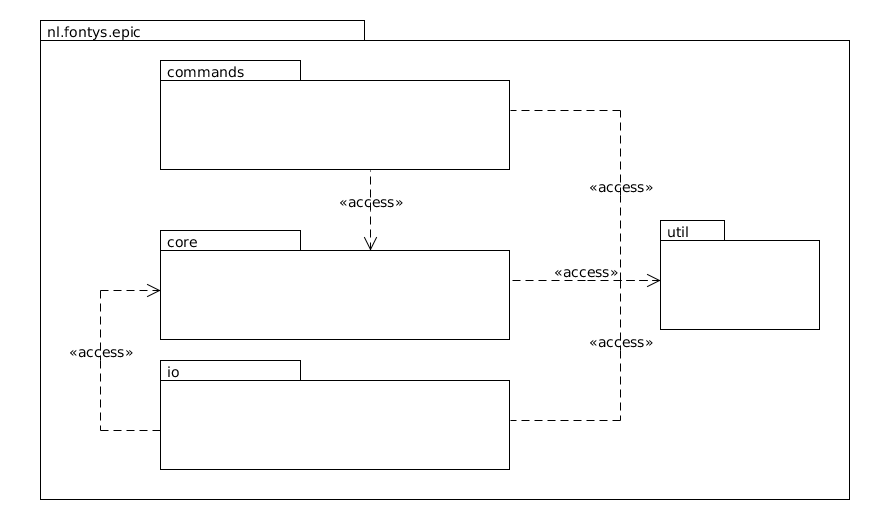
\includegraphics[scale=0.50]{assets/package-diagram.png}
IO-Package:

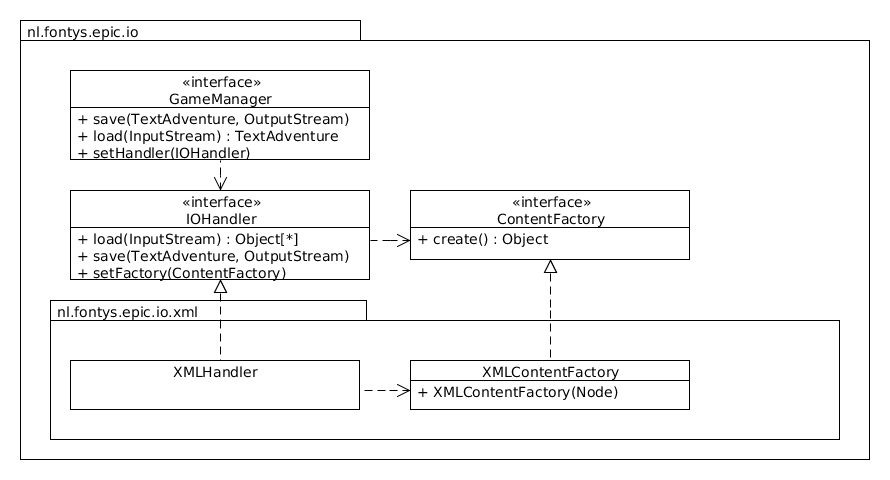
\includegraphics[scale=0.38]{assets/package-io.png}
CORE-Package

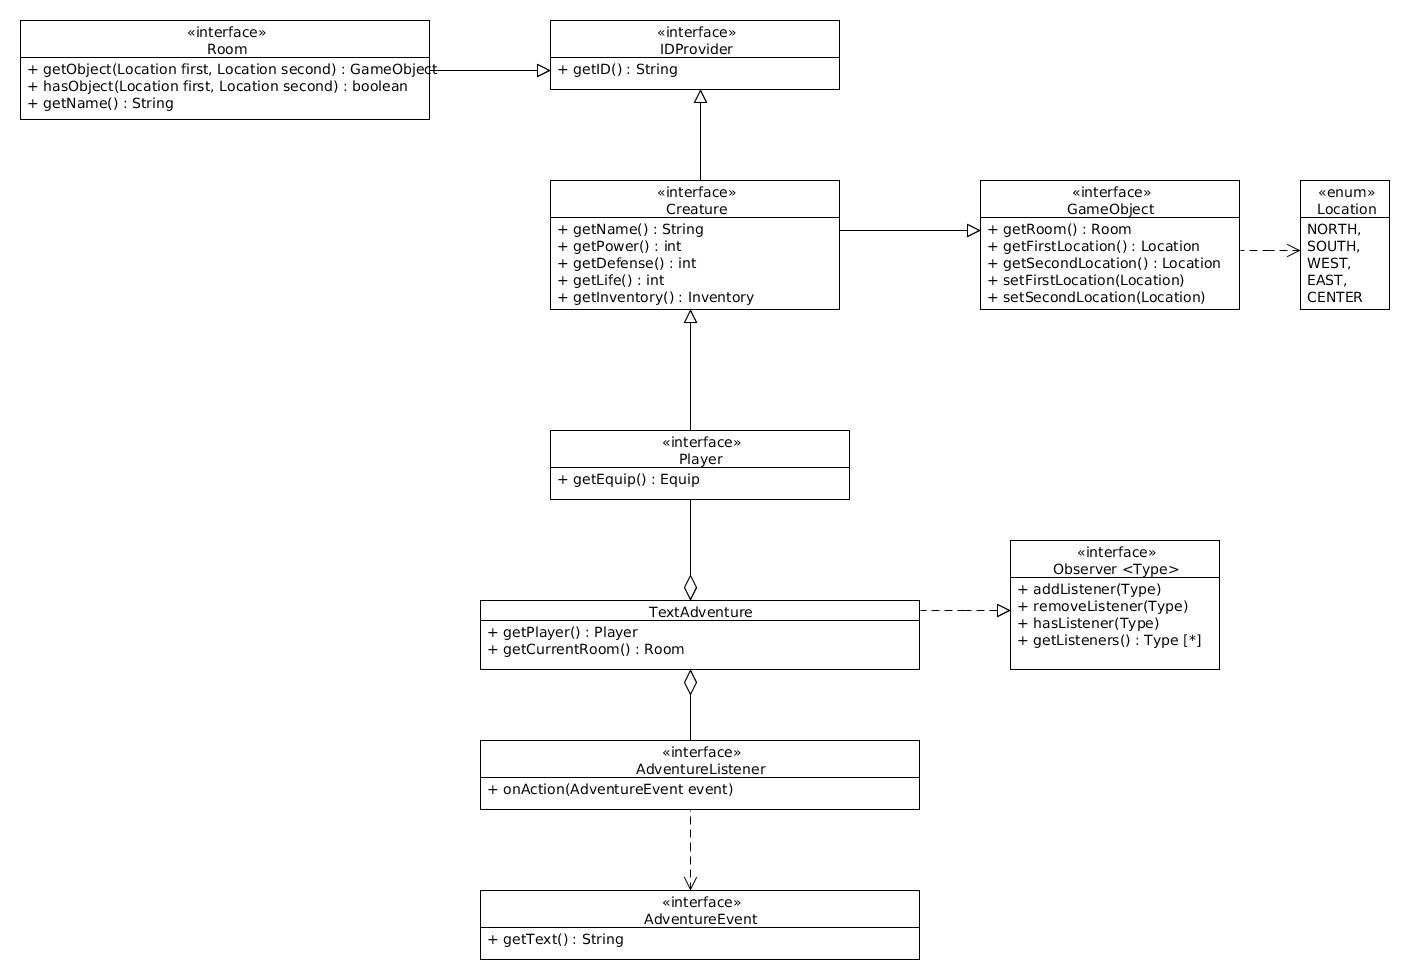
\includegraphics[scale=0.20]{assets/class-diagram.png}
